\section{Dezha Aidil Martha}
\subsection{Soal 1}
Buatlah librarri fungsi (file terpisah library dengan nama NPMbar.py) untuk plot dengan jumlah subplot adalah NPM mod 3 tambah 2

\lstinputlisting[firstline=8, lastline=38]{src/6/Praktek/1174025/d1174025_bar.py}

\subsection{Soal 2}
Buatlah librarri fungsi (file terpisah library dengan nama NPMscatter.py) untuk plot dengan jumlah subplot adalah NPM mod 3 tambah  2

\lstinputlisting[firstline=8, lastline=38]{src/6/Praktek/1174025/d1174025_scatter.py}

\subsection{Soal 3}
Buatlah librarri fungsi (file terpisah library dengan nama NPMpie.py) untuk plot dengan jumlah subplot adalah NPM mod 3 tambah 2

\lstinputlisting[firstline=8, lastline=61]{src/6/Praktek/1174025/d1174025_pie.py}

\subsection{Soal 4}
Buatlah librarri fungsi (file terpisah library dengan nama NPMplot.py) untuk plot dengan jumlah subplot adalah NPM mod 3 tambah  2

\lstinputlisting[firstline=8, lastline=38]{src/6/Praktek/1174025/d1174025_plot.py}
%%%%%%%%%%%%%%%%%%%%%%%%%%%%%%%%%%%%%%%%%%%%%%%%%%%5
\section{Habib Abdul Rasyid}
\subsection{Buatlah librari fungsi (file terpisah/library dengan nama NPM bar.py) untuk plot dengan jumlah subplot adalah NPM mod 3 + 2}
Subplot Grafik Bar dengan kodingan dan contoh sebagai berikut :

\lstinputlisting[firstline=11, lastline=27]{src/6/Praktek/1174002/1174002_bar.py}

\begin{figure}[h]
\centering
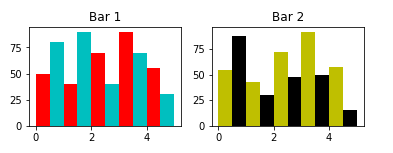
\includegraphics[scale=0.9]{figures/6/Praktek/1174002/npm_bar.png}
\caption{Hasil dari subplot Bar}
\label{fig:contoh}
\end{figure}

\subsection{Buatlah librari fungsi (file terpisah/library dengan nama NPM scatter.py) untuk plot dengan jumlah subplot NPM mod 3 + 2}

\lstinputlisting[firstline=8, lastline=35]{src/6/Praktek/1174002/1174002_scatter.py}

\begin{figure}[h]
\centering
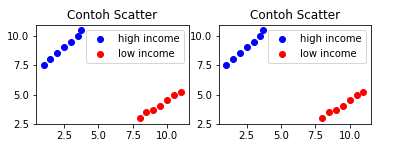
\includegraphics[scale=0.9]{figures/6/Praktek/1174002/scatter.png}
\caption{Hasil dari subplot Scatter}
\label{fig:contoh}
\end{figure}

\subsection{Buatlah librari fungsi (file terpisah/library dengan nama NPM pie.py) untuk plot dengan jumlah subplot NPM mod 3 + 2}

\lstinputlisting[firstline=8, lastline=51]{src/6/Praktek/1174002/1174002_pie.py}

\begin{figure}[h]
\centering
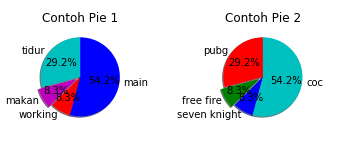
\includegraphics[scale=1.2]{figures/6/Praktek/1174002/pie.png}
\caption{Hasil dari subplot Pie}
\label{fig:contoh}
\end{figure}

\subsection{Buatlah librari fungsi (file terpisah/library dengan nama NPM plot.py) untuk plot dengan jumlah subplot NPM mod 3 + 2}

\lstinputlisting[firstline=8, lastline=23]{src/6/Praktek/1174002/1174002_plot.py}

\begin{figure}[h]
\centering
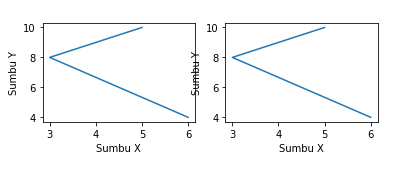
\includegraphics[scale=0.9]{figures/6/Praktek/1174002/plot.png}
\caption{Hasil dari subplot Plot}
\label{fig:contoh}
\end{figure}

\subsection{Isi File main untuk mengimport dan running kodingan diatas}

\lstinputlisting[firstline=7, lastline=18]{src/6/Praktek/1174002/main.py}
%%%%%%%%%%%%%%%%%%%%%%%%%%%%%%%%%%%%%%%%%%%%%%%%55

